\section{Testing}
In this section we will briefly describe how we tested the application following the general guideline given in the Design Document.\\
We decide to test only the backend because the frontend just display the data received from the backend.

\subsection{Integration tests}
\begin{itemize}
    \item \textbf{DiscussionIntegrationTest:} we tested the discussion controller methods. First of all we created a new discussion with a post, then we deleted another one and tried to delete a discussion not present  and finally tried to update another discussion. We tested also the methods that fetch the discussions, searching for the the discussion published by a policy maker (also for a policy maker that does not have publish any discussion yet), the most active discussions in the forum and we implemented a test to retrieve the users that follows a discussion.
    \item \textbf{PostIntegrationTest:} we tested the methods linked to the posts. We tried to insert a new post using a Policy maker account and a user account, then we tried to delete and update them, we tested the approve and the decline pending post methods and we repeat the same tests with non valid input or authorizations to see if the error would be catched.
    \item \textbf{UserIntegrationTest:} we tested the user controller methods. First of all, we created a new Policy maker account and one for a user, then we tried to search an account not present in the database and after that we updated a User account. Eventually we tested the method to retrieve the most active users.
    \item \textbf{DataIntegrationTest:} we tested the data related methods. We tried to fetch data for a not existing district, then we created rankings for different districts and retrieved all the data available for a single district. We fetched data from a given data set and finally we calculated the ranking list for a set of districts selecting the data sources of interest.
\end{itemize}

\subsection{Testing results}

\begin{figure}[h!]
    \centering
    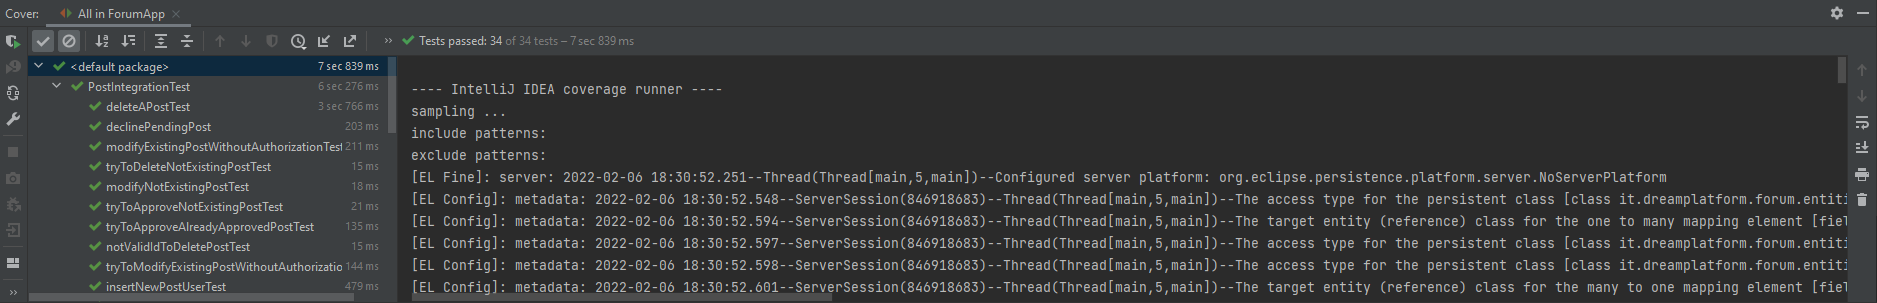
\includegraphics[scale=0.25]{images/testing/testing_forum.png}
    \caption{Forum testing results}
    \label{fig:forum_testing}
\end{figure}
\FloatBarrier

\begin{figure}[h!]
    \centering
    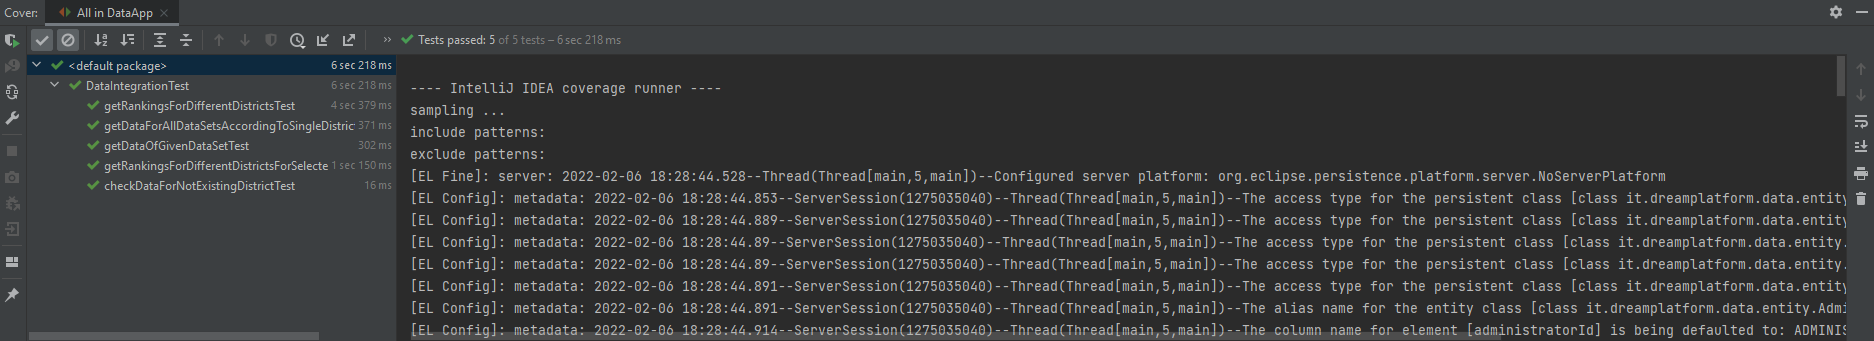
\includegraphics[scale=0.25]{images/testing/testing_data.png}
    \caption{Data testing results}
    \label{fig:data_testing}
\end{figure}
\FloatBarrier

\subsection{Testing coverage}

\begin{figure}[h!]
    \centering
    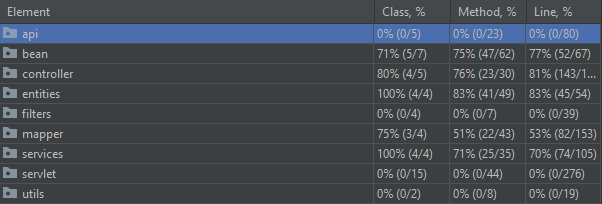
\includegraphics[scale=0.50]{images/testing/coverage_forum.png}
    \caption{Forum testing coverage}
    \label{fig:forum_coverage}
\end{figure}
\FloatBarrier

\begin{figure}[h!]
    \centering
    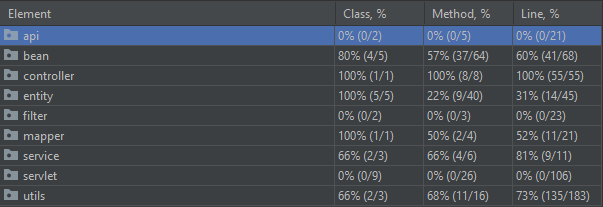
\includegraphics[scale=0.50]{images/testing/coverage_data.png}
    \caption{Data testing coverage}
    \label{fig:data_coverage}
\end{figure}
\FloatBarrier